\documentclass[conference]{IEEEtran}
\IEEEoverridecommandlockouts

%\usepackage{cite}
\usepackage{amsmath,amssymb,amsfonts}
\usepackage{algorithmic}
\usepackage{graphicx}
\usepackage{natbib}
\usepackage{textcomp}
\usepackage{xcolor}
\def\BibTeX{{\rm B\kern-.05em{\sc i\kern-.025em b}\kern-.08em T\kern-.1667em\lower.7ex\hbox{E}\kern-.125emX}}

\begin{document}
\bibliographystyle{IEEEtran}

\title{An Efficiency of Third Party Genetic Algorithms Software Libraries in Mobile Distributed Computing for Financial Time Series Forecasting\\
{\footnotesize \textsuperscript{}}
\thanks{This research is funded by Velbazhd Software LLC.}
}

\author{\IEEEauthorblockN{1\textsuperscript{st} Gergana Mateeva}
\IEEEauthorblockA{\textit{Institute of Information and Communication Technologies} \\
\textit{Bulgarian Academy of Sciences}\\
Sofia, Bulgaria \\
gergana.mateeva@iict.bas.bg}
\and
\IEEEauthorblockN{2\textsuperscript{nd} Dimitar Parvanov}
\IEEEauthorblockA{\textit{Institute of Information and Communication Technologies} \\
\textit{Bulgarian Academy of Sciences}\\
Sofia, Bulgaria \\
dimitar.parvanov@iict.bas.bg}
\and
\IEEEauthorblockN{3\textsuperscript{rd} Ioan Dimitrov}
\IEEEauthorblockA{\textit{Faculty of Electronic Engineering and Technology} \\
\textit{Technical University of Sofia}\\
Sofia, Bulgaria \\
joancdimitrov@tu-sofia.bg}
\and
\IEEEauthorblockN{4\textsuperscript{th} Iliyan Iliev}
\IEEEauthorblockA{\textit{Institute of Information and Communication Technologies} \\
\textit{Bulgarian Academy of Sciences}\\
Sofia, Bulgaria \\
iliyan.iliev@iict.bas.bg}
\and
\IEEEauthorblockN{5\textsuperscript{th} Todor Balabanov}
\IEEEauthorblockA{\textit{Institute of Information and Communication Technologies} \\
\textit{Bulgarian Academy of Sciences}\\
Sofia, Bulgaria \\
todor.balabanov@iict.bas.bg}
}

\maketitle

\begin{abstract}
Genetic algorithms are very well-known optimization meta-heuristics. They are very well presented in mathematical applications like Matlab, R, and others. Such specific implementations are not proper for industrial software development. Because of its popularity, genetic algorithms have become implemented as third-party software libraries. The popularity of Android OS with its capabilities for running Java source code attracted the usage of external software libraries for achieving mobile distributed computing tasks. Training of artificial neural networks and curve fitting by the usage of genetic algorithms brought financial time series forecasting to the mobile world. In this study, two of the most popular genetic algorithm software libraries are compared in order to be used in mobile distributed computing application.
\end{abstract}

\begin{IEEEkeywords}
genetic algorithms, mobile distributed computing, software libraries
\end{IEEEkeywords}

\section{Introduction}

In the face of mobile distributed computing \cite{Bibi-2021-a}, state of the art in soft computing \cite{Angelova-2009-a} received a valuable extension. Additional acceleration of mobile device usage adoption has been given by Covid-19 pandemic \cite{Petrov-2021-a}. Wireless sensor networks \cite{Alexandrov-2016-a} in combination with smart routing \cite{Tashev-2019-a} and IoT \cite{Dineva-2019-a} were a valuable idea source for mobile distributed computing implementations. The usage of heterogeneous devices \cite{Weinbub-2012-a}  appears to be very efficient for slipping calculations in complex combinatorial problems \cite{Borissova-2015-a}. When calculating devices are in a volunteer scheme the control over them is unknown \cite{Balabanov-2020-a}, which leads to a number of cybersecurity issues \cite{Dimitrov-2021-a}. 

In this study, a mobile distributed computing software \cite{Balabanov-2022-a} has been extended. The extension comes to the machine learning algorithms applied in financial time series forecasting. Two of the most popular software libraries for genetic algorithms are included (MOEA Framework \cite{Huo-2018-a} and Jenetics \cite{Aalam-2022-a}). 

The paper is organized as follows: Section 2 introduces mobile distributed computing and its specifics; Section 2 presents financial time series forecasting and some of the related challenges; Section 3 reveals some experiments and results; Section 4 concludes and provides some guidance for further research.

\section{Distributed Computing}

Only a limited number of computational problems are proper for distributed computing. The main condition for this suitability is the presence of calculating instructions that can be performed simultaneously \cite{Hillis-1986-a}. When it comes to computers in a global network, it is useful for the synchronization of the results to be done less frequently than in parallel computing. 

For example, the parallel implementation of the QuickSort \cite{Sanders-1997-a} algorithm is not proper as distributed computing implementation. Partially sorted sub-arrays need strong synchronization during the parallelization process. In distributed computing, it is very common for some calculating nodes to disappear from the network without any warning. If such an event happens during a parallel run of QuickSort the whole calculation would fail. Because of these reasons, algorithms like QuickSort are proper for multiprocessor machines with common memory but are not proper for distributed computing. 

On the other side, evolutionary algorithms \cite{Sudholt-2015-a} have a very high degree of parallelism. Intermediate calculations in evolutionary algorithms are mainly useless. Losing some intermediate results does not affect too much the final outcome. In distributed computing implementation of some evolutionary algorithms, there is a very low need for synchronization. All described making evolutionary algorithms a perfect option for doing distributed computing. 

In most cases, evolutionary algorithms themselves are very fast performing \cite{Vural-2012-a}. The low performance comes when the target function (fitness value calculation) is computationally time-consuming \cite{Di-Pietro-2004-a}. For their effectiveness, most of the evolutionary algorithms do perform a lot of calculations of the target function  \cite{Shi-2010-a}. It is needed because many different candidate solutions should be checked or involved in the optimization process. When both factors come together, too many calculations of a very time-consuming target function, the optimization becomes practically unusable \cite{Lee-2015-a}. 

All mentioned above lead to the logical conclusion that distributed computing perfectly fits the needs of low-performing evolutionary algorithms. A global population of solutions is handled on a very low resource usage remote server \cite{Gong-2015-a}. The server does mainly storage and less frequent synchronization with the calculating nodes. Because calculating nodes are highly independent, a local evolution of the solutions can be done for a long period of time without the need for synchronization. 

\section{Time Series Forecasting}

Vitosha Trade Android Client \cite{Balabanov-2022-a} is a mobile distributed computing application. It uses the capabilities of the Android OS as visualization and background calculations. The application is partially under development in the Institute of Information and Communication Technologies as part of the Bulgarian Academy of Sciences. The main goal of the project is financial time series forecasting \cite{Kolarik-1994-a}. It is achieved by gradient-based methods for artificial neural networks training \cite{Tomov-2021-a} and evolutionary algorithms \cite{Tomov-2021-b}. Android services are used as tools for doing calculations in the background. Visualization of the intermediate results is done with Android live wallpaper capabilities \cite{Mateeva-2021-a}. 

Mobile distributed computing in this project is organized as client-server \cite{Sinha-1992-a} software architecture. Time series are provided from a light-weighted remote web server. A global population of solutions is also available through the same server. Mobile devices connect to the server, as RESTful communication \cite{Orellana-2012-a}, and through HTTP/JSON protocol request calculating packages. 

Global population and local populations are subsets of artificial neural networks weights matrices. Local populations are handled by different evolutionary algorithms, in some cases genetic algorithms. Individuals of the local populations are loaded in an artificial neural network structure when the fitness value is calculated. Such calculation is very time-consuming because the artificial neural network performs all input-output examples and the root mean square error is calculated. 

In addition to the artificial neural networks, a second approach for financial time series forecasting is also used. It is based on sine series curve fitting \cite{Iliev-2021-a}. The trend of the financial time series is approximated with an equation of a line. The sum of the sine functions approximates the fluctuations in the financial times series. A genetic algorithm is applied to search for near-optimal solutions of the coefficients used for the line equation the sine functions. Chromosomes consist of two coefficients for the line function and three coefficients for each sine function. The goal of the optimization is for the resulting curve to be as close to the original points as possible. 

\section{Experiments \& Results}

Experiments have been done with both frameworks for doing nonlinear curve fitting with a single line and a sum of nine sine functions. The price of Bitcoin in US dollars is taken as experimental data (Fig. \ref{fig01}).

\begin{figure}[htbp]
\centerline{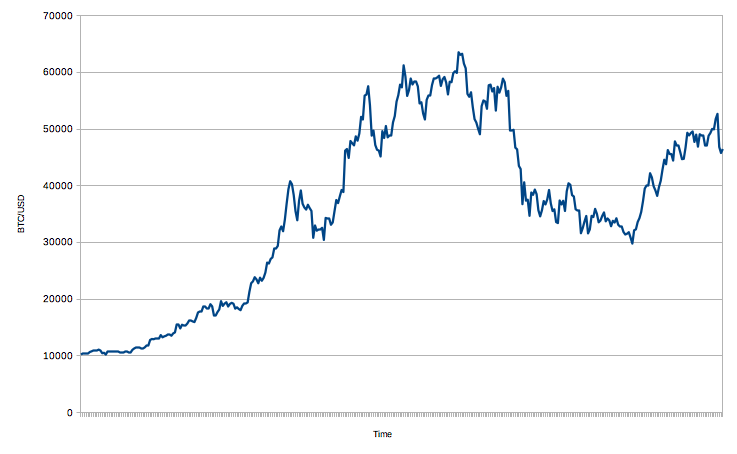
\includegraphics[width=8.4cm]{fig01.png}}
\caption{Bitcoin price.}
\label{fig01}
\end{figure}

All calculations have been done on Intel Core i5 2.3GHz, a single CPU with 2 cores, 8GB RAM, macOS High Sierra 10.13.6, Java SE
11.0.2, MOEA Framework 2.13, and Jenetics 7.0.0. The population of the genetic algorithms was selected to be 137 individuals. Tournament selection with an elitism rule has been used. A crossover rate of 95\% and a mutation rate of 1\% were preferred. Evolution time was selected to be 60 seconds with measurements of the progress on each second. 

\begin{figure}[htbp]
\centerline{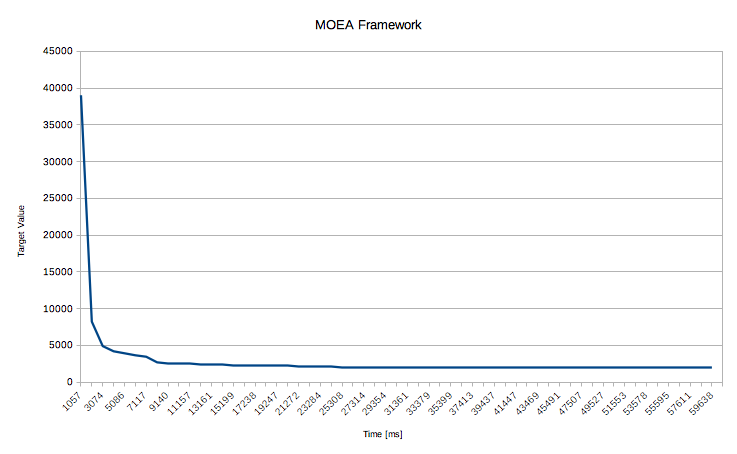
\includegraphics[width=8.4cm]{fig02.png}}
\caption{MOEA Framework convergence.}
\label{fig02}
\end{figure}

\begin{figure}[htbp]
\centerline{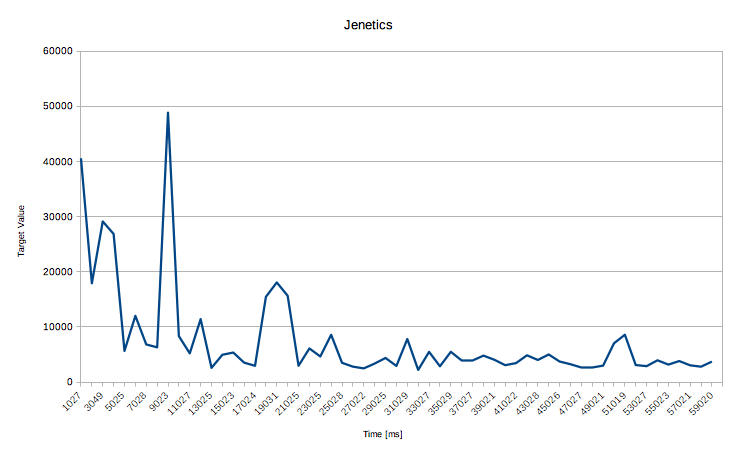
\includegraphics[width=8.4cm]{fig03.png}}
\caption{Jenetics convergence.}
\label{fig03}
\end{figure}

As convergence, the lower point was achieved by MOEA Framework (Fig. \ref{fig02}), where Jenetics convergence is less smooth (Fig. \ref{fig03}), showing clearly that the process is less stable. MOEA Framework was able to make almost twice more target function (Fig. \ref{fig04}) calculations than Jenetics (Fig. \ref{fig05}). In a general conclusion, MOEA Framework is much easier to use, has more stable convergence and performance is much better.

\begin{figure}[htbp]
\centerline{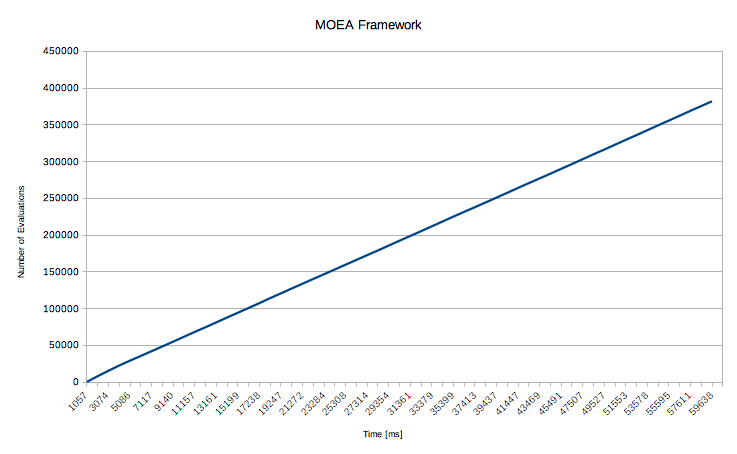
\includegraphics[width=8.4cm]{fig04.png}}
\caption{MOEA Framework number of target function calculations.}
\label{fig04}
\end{figure}

\begin{figure}[htbp]
\centerline{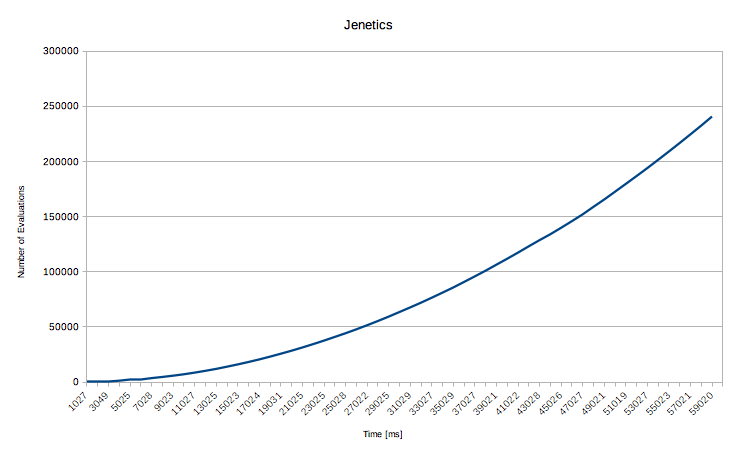
\includegraphics[width=8.4cm]{fig05.png}}
\caption{Jenetics number of target function calculations.}
\label{fig05}
\end{figure}

\section{Conclusion}

In this study, the efficiency of the MOEA Framework and Jenetics framework were compared, when they are used for genetic algorithms optimization in financial time series forecasting. As a result of the experiments done, MOEA performs much faster than Jenetics. The too complicated object-oriented implementation of Jenetics makes it extremely difficult to use. The objects in Jenetics are immutable which gives good thread safety but dramatically affects its performance. Both libraries are written in Java, but code compliance with Android can be challenging. 

In further research, other software libraries can be investigated and compared with those already included in the project.

\section*{Acknowledgment}

This research is funded by Velbazhd Software LLC. It is partially supported by the Ministry of Education and Science of the Republic Bulgaria under the National Science Program “Intelligentanimal husbandry”, grant agreement No. D01-62/18.03.2021/, the National Research Programme “Young scientists and postdoctoral students” approved by DCM No. 577/17.08.2018, and the Bulgarian National Science Fund by the project “Mathematical models, methods and algorithms for solving hard optimization problems to achieve high security in communications and better economic sustainability”, KP-06-N52/7/19-11-2021.

\bibliography{references}

\end{document}
